% The following answers were used to create this image:
% - http://tex.stackexchange.com/a/45824/5645 - Grid
% - http://tex.stackexchange.com/a/373/5645 - Torus
\documentclass[border=2pt]{standalone}
\usepackage{amsmath,amssymb}
\usepackage{tikz}
\usetikzlibrary{patterns,arrows,positioning}

\begin{document}
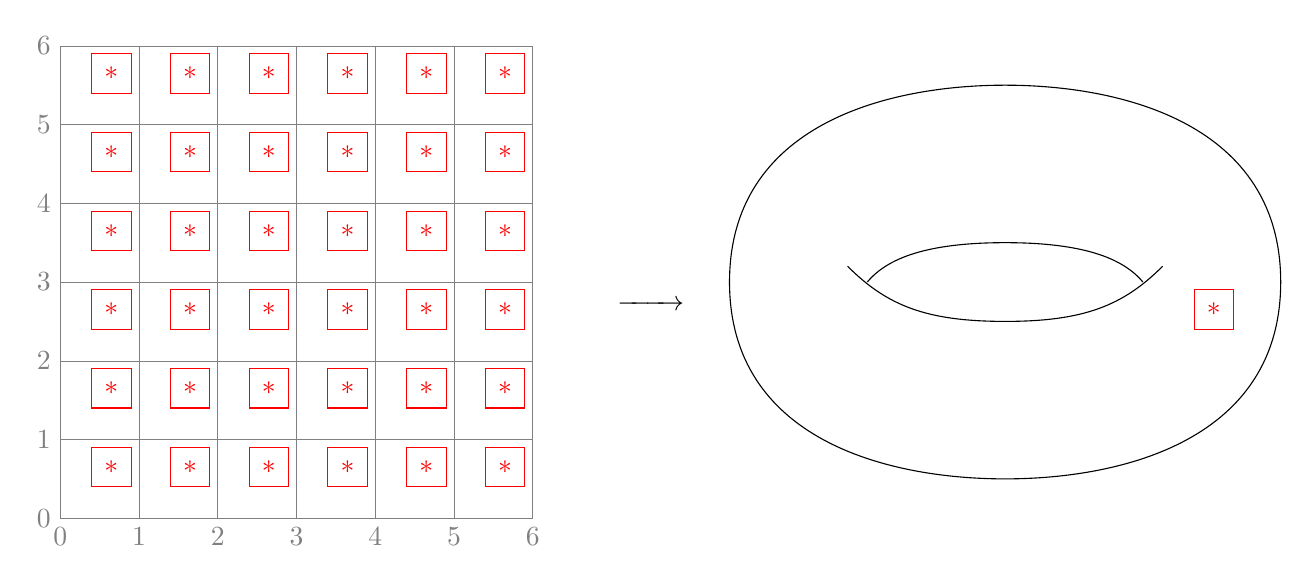
\begin{tikzpicture}
\tikzstyle{point}=[circle,thick,draw=black,fill=black,inner sep=0pt,minimum width=4pt,minimum height=4pt]
\newcommand*{\xMin}{0}%
\newcommand*{\xMax}{6}%
\newcommand*{\yMin}{0}%
\newcommand*{\yMax}{6}%

\draw (-3.5,0) .. controls (-3.5,2) and (-1.5,2.5) .. (0,2.5);
\draw[xscale=-1] (-3.5,0) .. controls (-3.5,2) and (-1.5,2.5) .. (0,2.5);
\draw[rotate=180] (-3.5,0) .. controls (-3.5,2) and (-1.5,2.5) .. (0,2.5);
\draw[yscale=-1] (-3.5,0) .. controls (-3.5,2) and (-1.5,2.5) .. (0,2.5);

\draw (-2,.2) .. controls (-1.5,-0.3) and (-1,-0.5) .. (0,-.5) .. controls (1,-0.5) and (1.5,-0.3) .. (2,0.2);
\draw (-1.75,0) .. controls (-1.5,0.3) and (-1,0.5) .. (0,.5) .. controls (1,0.5) and (1.5,0.3) .. (1.75,0);


\begin{scope}[shift={(-12,-3)}]
    \foreach \i in {\xMin,...,\xMax} {
        \draw [very thin,gray] (\i,\yMin) -- (\i,\yMax)  node [below] at (\i,\yMin) {$\i$};
    }
    \foreach \i in {\yMin,...,\yMax} {
        \draw [very thin,gray] (\xMin,\i) -- (\xMax,\i) node [left] at (\xMin,\i) {$\i$};
    }

    \begin{scope}[shift={(14,2)}]
        \node (P) at (0.4,0.9) {};
        \node (Q) at (0.9,0.4) {};
        \draw [red] (P) rectangle (Q);
        \draw (0.65, 0.6) node[red] {*};
    \end{scope}

    \foreach \x in {0,1,2,3,4,5} {
        \foreach \y in {0,1,2,3,4,5} {
            \begin{scope}[shift={(\x,\y)}]
                \node (P) at (0.4,0.9) {};
                \node (Q) at (0.9,0.4) {};
                \draw [red] (P) rectangle (Q);
                \draw (0.65, 0.6) node[red] {*};
            \end{scope}
        }
    }
\end{scope}
    \draw (-4.5, 0) node[below] {$\xrightarrow{\text{\;\;\;\;\;\;\;\;}}$};
\end{tikzpicture}
\end{document}
